\section{Введение}
Фермент фруктозодифосфатальдолаза (EC 4.1.2.13) катализирует обратимое расщепление
фруктозо-1,6-дифосфата между $C_3$ и $C_4$ с образованием диоксиацетонфосфата и глицеральдегидфосфата.
Равновесие сильно сдвинуто в направлении обратной реакции.
Данная реакция является частью гликолиза. Также фермент участвует в гликонеогенезе;
было доказано, что иногда он может функционировать как адапторный белок.

Реакция образования глицеральдегид-3-фосфата и дигидроксиацетонфосфата:\\
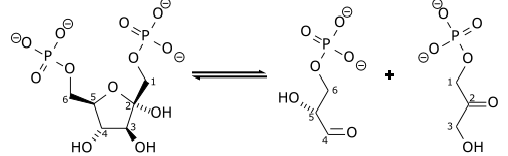
\includegraphics[width=0.8\linewidth]{intro-react}

Фермент представляет собой тетрамер, состоящий из 4 одинаковых субъединиц
($ 162 \text{kDa} = 4 \cdot 40.5 \text{kDa} $).
Животные ткани содержат по меньшей мере три различные альдолазы, характерные для
мышцы, печени и мозга (A, B, C).

Пространственная структура альдолазы А из мышц кролика, рисунок был взят из банка данных PDB, код - 1ZAH:\\
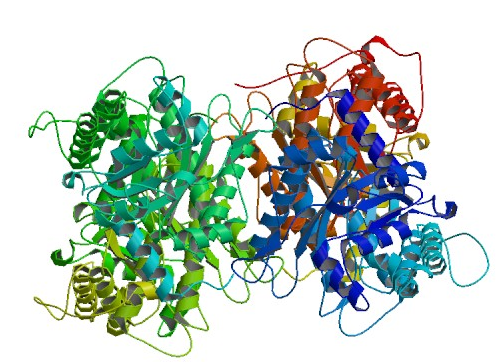
\includegraphics[width=0.8\linewidth]{intro-pdb}

A, B, C кодируются тремя разными генами и по-разному экспрессируются в течение развития организма.
Альдолазы А и С были найдены в тканях взрослых животных.

\emph{Кинетические параментры}: для человека константа Михаэлиса Km=52 µM для фруктозо-1,6-бисфосфата
(информация была взята с Uniprot, P04075, ALDOA\_HUMAN).

